\section{Synapsed}

\begin{frame}{Introduction}
	Previous results show that:
	\begin{itemize}
		\item There is high lock contention
		\item The amount of RAM is important
	\end{itemize}
	\note[item]{Από τα προηγούμενα συμπεράσματα, μπορούμε να εξάγουμε ότι 
		έχουμε τα εξής limitations ανεξαρτήτως latency Αρχιπελάγους: 
		lock contention και έλλειψη από RAM}
	\dspc
	If cached remains at the host, it will:
	\begin{itemize}
		\item Compete for CPU time
		\item Use a fraction of the host's RAM
	\end{itemize}
	\note[item]{Αν ο cached τρέχει στον host όπου τρέχουν και τα VMs, θα 
		έχουμε λιγότερη cpu -> περισσότερο contention και λιγότερη ram}
	\dspc
	Idea: what if cached ran on storage nodes?
	\note[item]{Αν έτρεχε στους αποθηκευτικούς κόμβους;}
\end{frame}

\begin{frame}
	If cached was on storage nodes, the pros would be:
	\begin{itemize}
		\item Access to more RAM
		\item Major step towards a distributed cache
	\end{itemize}
	\note[item]{Αν έτρεχε εκεί θα \todo}
	\dspc
	On the other hand, the cons would be:
	\begin{itemize}
		\item Network bottleneck
		\item Bigger complexity
	\end{itemize}
	\dspc
	Archipelago is network-unaware. Must create a proof-of-concept network peer 
	to help us in this task.
\end{frame}

\begin{frame}{Synapsed design}
	Synapsed is designed to do the following:
	\begin{itemize}
		\item Connect two Archipelago peers over network
		\item Forward read/write XSEG requests
		\item Use the TCP protocol
		\item Integrate with the Archipelago signaling mechanism
		\item Use zero-copy methods
	\end{itemize}
	\dspc
	Replication should be trivial to implement, but it is currently missing.

	\note[item]{Το synapsed σχεδιάστηκε για τα εξής:
		\begin{itemize}
			\item Σύνδεση δυο Αρχιπέλαγο peers πάνω από network
			\item Κατάλληλη προώθηση I/O αιτημάτων
			\item Χρήση του tcp πρωτοκόλλου
			\item Χρήση του signaling μηχανισμού του Αρχιπελάγους
			\item Χρήση μεθόδων zero-copy
		\end{itemize}
	}
	\note[item]{H δημιουργία αντιγράφων μπορεί να προστεθεί εύκολα στα 
		παραπάνω, αλλά εμείς δεν φτάσαμε ώς εκει}

\end{frame}

\begin{frame}{Benchmark preamble}
	The most important part is that synapsed works. We are \textbf{now} able to
	run cached or part of Archipelago in the storage nodes.
	\dspc
	However, let's check its performance.
	\spc
	We will attempt to run most of the previous scenarios using synapsed this 
	time.
	\dspc
	Note, synapsed is proof-of-concept and not performance-tuned. Also, the 
	tested configuration uses a 1Gbit connection.
	\note[item]{O κύριως στόχος του synapsed είναι να προσφέρει τη 
		δυνατότητα ή ελαστικότηατα αν το θέλετε, του να τρέχει ο cached 
		ή κομματι του Archipelago σε άλλο κόμβο. Ας δούμε όμως την 
		επίδοσή του
	}
\end{frame}

\begin{frame}{Synapsed results}
	\begin{columns}[t]
		\begin{column}{.5\textwidth}
			Write bandwidth
			\makebox[\textwidth]{
				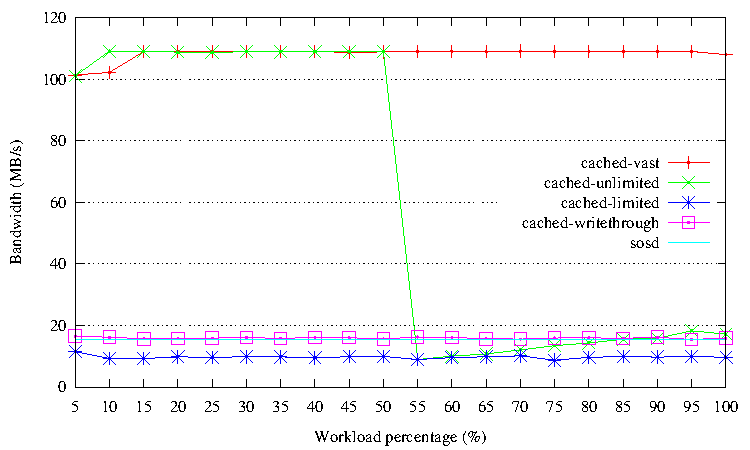
\includegraphics[width=\columnwidth]{images/bw-write-synapsed.pdf}
			}
			Constants:
			\begin{itemize}
				\item cached has 4 threads
				\item workload twice the cache size
				\item block size is 4KB
				\item Parallel requests are 16
			\end{itemize}
		\end{column}
		\begin{column}{.5\textwidth}
			Write latency
			\makebox[\textwidth]{
				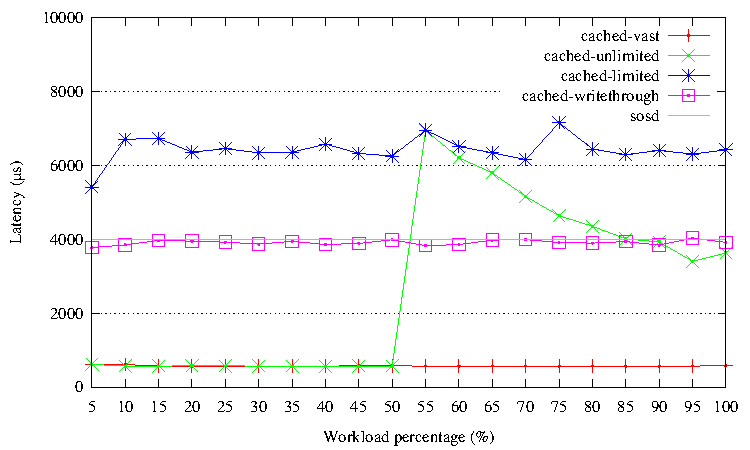
\includegraphics[width=\columnwidth]{images/lat-write-synapsed.pdf}
			}
			Variables:
			\begin{itemize}
				\item cache write policy
				\item maximum cached objects
			\end{itemize}
		\end{column}
	\end{columns}
	\note{Σημεία προσοχής, πρακτικά υπάρχει πολύ μικρή διαφορά με το 
		διάγραμα της σελίδας 32. Απλά μπάινει μικρότερο του 1ms latency 
		που για το cached-vast φυσικά κάνει μεγάλη διαφορά.\dspc
		Κατά τα άλλα, το latency αυτό είναι αμελητέο σε σχέση με το 
		τρέχων latency, ενώ αν υπήρχε 10 ή 40Gbit δίκτυο, θα ήταν ακόμα 
		καλύτερα τα πράγματα.
	}
\end{frame}

